
\documentclass{standalone}
\usepackage[T1]{fontenc}
\usepackage[utf8]{inputenc}
\usepackage{pgf,tikz}
\usepackage{amsmath}

\begin{document}

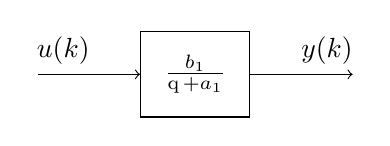
\begin{tikzpicture}[node distance=20mm, anchor=north]
   \node[coordinate] (input) {};
   \node[rectangle, draw, right of=input, inner sep=3mm] (lti) {$\frac{b_1}{\operatorname{q} + a_1}$};
   \node[coordinate, right of=lti] (output) {};
   \draw[->] (input) -- node[near start, above] {$u(k)$}  (lti);
   \draw[->] (lti) -- node[near end, above] {$y(k)$} (output);
 \end{tikzpicture}
\end{document}
